%% Präambel
%% Initialisierung
%% Pakete laden

%% Format der Arbeit
\documentclass[enabledeprecatedfontcommands, a4paper, twoside]{scrreprt}    % articel: scrartcl   % book: scrreprt
% für einseitigen Druck (kein Buchformat) "twoside" entfernen
% für A5 Format "a5paper" verwenden
\usepackage[T1]{fontenc}
\usepackage[utf8]{inputenc}
\usepackage{fancyhdr}

%% Sprache
\usepackage[ngerman]{babel}

%% Boxstyle
\usepackage{fancybox}

%% Fußnoten
\usepackage{endnotes}

% Lesezeichenpacket für PDF
\usepackage{hyperref}

%% American Mathematical Society Pakete
\usepackage{amsmath,esint}
\usepackage{amsfonts}
\usepackage{amssymb}
\usepackage{amstext}
\usepackage{mathrsfs}
\usepackage{bbm}
\usepackage{cancel}
\DeclareMathAlphabet\mathbfcal{OMS}{cmsy}{b}{n}
\usepackage{trfsigns}

%% Grafik Paket
\usepackage{graphicx}
\usepackage{float}

%% Optional: Subfigures (mehrere Unterabbildungen in einer figure)
\usepackage{subfig}

%% Paket zum Einfügen von Quellcode (Sprache kann hier definiert werden)
\usepackage{listings}
\lstset{
	language = C++,
	showstringspaces = false,
	numbers = left,
	breaklines = true,
}

%% Zeileneinrücken verhindern
\setlength{\parindent}{0em} 

%% optional: Randlose Kapitelmarker (Daumenregister)
% Zur Verwendung für neue Kapitel \thumbchapter anstelle von \chapter verwenden
\usepackage{thumbs}
\pagenumbering{arabic}
\newcommand{\thumbchapter}[1]{
	\chapter{#1}
	\addthumb{#1}{
		\space\Huge\sffamily\bfseries \thechapter}{black}{lightgray}
}

%% optional: Quellenangabe von Bildern direkt unter der Grafik
% Zur Verwendung für Bildquellen \bildquelle verwenden
\newcommand*{\bildquelle}[1]{\par\raggedleft\footnotesize Quelle:~#1}

%% optional: Erlaubt Formatierung von Dateipfaden mit \path und URLs mit \url
\usepackage{url}

%% optional: Breiterer Rand außen
\usepackage[left=2.5cm, right=5cm, top=2.5cm, bottom=2.5cm]{geometry}

%% optional: Booktabs für schönere Tabellen
\usepackage{booktabs} % Für schöneres Tabellenaussehen

%% Style
\pagestyle{fancy}
\lhead[\bfseries \title \protect]{\bfseries \title \protect}

%% Format der Bibliographie
\usepackage{natbib}
\bibliographystyle{alpha} % Harvard Zitierweise (Autorenkürzel für Quellen)
%\bibliographystyle{abbrv} % Deutsche Zitierweise (Ziffern für Quellen)

\begin{document}

%% Titelseite einfügen
\begin{titlepage}
{\centering

\includegraphics[width=0.6\textwidth]{HS_Logo2}\par
\vspace{1cm}
{\scshape\LARGE University of Applied Sciences Trier \par}
\vspace{1.5cm}
{\scshape\Large Master Thesis \par}
\vspace{1.5cm}
{\huge\bfseries Themenbeschreibung der Arbeit \par}
\vspace{1.5cm}
{\scshape \large Master of Science \par}
\vspace{0.8cm}
{\scshape\large Elektrotechnik\par}
{\scshape\large Informationstechnologie und Elektronik  \par}
\vspace{1.5cm}
{verfasst von: \\  \par}
%\vspace{0.2cm}
{\large  Andreas  \textsc{Reis}, B. Eng.\\  \par}
 \vspace{0.5cm}
betreut von: \par
{\large Prof. Dr. rer. nat. Ernst Georg \textsc{Haffner} \\  Prof. Dr. Matthias \textsc{Scherer} \par}
\vspace{0.5cm}
{Abgabedatum: \\  \par}
{\large \today \par}} %\today
\end{titlepage}

\cleardoublepage
	
%% Eidesstattliche Erklärung
{\huge \textbf{Eidesstattliche Erklärung}} \\ \\
Ich versichere, die vorliegende Arbeit selbstständig und lediglich unter Benutzung der angegebenen Quellen und Hilfsmittel verfasst zu haben. \\

Alle Stellen, die wörtlich oder sinngemäß aus veröffentlichten oder noch nicht veröffentlichten Quellen entnommen sind, sind als solche kenntlich gemacht. Die Zeichnungen oder Abbildungen in dieser Arbeit sind von mir selbst erstellt worden oder mit einem entsprechenden Quellennachweis versehen. \\

Ich erkläre weiterhin, dass die vorliegende Arbeit noch nicht im Rahmen eines anderen Prüfungsverfahrens eingereicht wurde. \\ \\ \\

\begin{center}
	\vspace{1.5cm}
	\begin{tabular}{lp{2em}l}
		\hspace{5cm}   && \hspace{5cm} \\
		\cline{1-1}\cline{3-3}
		Ort, Datum  && \hfill Unterschrift
	\end{tabular} 
\end{center}

\newpage

%% Abstract
{\huge{\textbf{Abstract}}}\\

Diese Arbeit ist eine Vorlage für zukünftige Abschluss- / Projektarbeiten.

\clearpage

{\huge{\textbf{Abstract (English)}}}\\

% Anmerkung: Ich empfehle Deepl als Übersetzer (www.deepl.com)
This paper is a template for future final / project papers.


%% Inhaltsverzeichnis
\cleardoublepage\pdfbookmark{\contentsname}{toc}\tableofcontents
\newpage

%% Glossar
% Diese Vorlage kann auch für andere Verzeichnisse verwendet werden, zum Beispiel für Formelverzeichnis

\chapter*{Glossar}
\addcontentsline{toc}{chapter}{Glossar}
% Die Begriffe sollten alphabetisch sortiert werden
\begin{table}[H]
	\begin{center}
		\begin{tabular}{ c | c}
			\parbox[c][0.8cm][c]{.3\linewidth}{\centering\textbf{Begriff} } 
			& 
			\parbox[c][0.8cm][c]{.6\linewidth}{\centering\textbf{Definition}}
			\\
			\hline %%%%%%%%%%%%%%%%%%%%%%%%%%%%%%%%%%%%%%%%%%%
			\hline %%%%%%%%%%%%%%%%%%%%%%%%%%%%%%%%%%%%%%%%%%%
			\parbox[c][0.8cm][c]{.3\linewidth}{\centering Eintrag 1 }  
			& 
			\parbox[c][0.8cm][c]{.6\linewidth}{\centering Definition 1}
			\\ 
			\hline %%%%%%%%%%%%%%%%%%%%%%%%%%%%%%%%%%%%%%%%%%%
			\parbox[c][0.8cm][c]{.3\linewidth}{\centering Eintrag 2 }  
			& 
			\parbox[c][0.8cm][c]{.6\linewidth}{\centering Definition 2}
			\\ 
		\end{tabular}
	\end{center}
\end{table}


%% Abbildungs- und Tabellenverzeichnis %%%%%%%%%%%%%%%%%%%%%%%%%%%%%%%%%%%%%%%%%%%%%%%%
\newpage
\noindent
\listoffigures
\addcontentsline{toc}{chapter}{Abbildungsverzeichnis}
\listoftables
\addcontentsline{toc}{chapter}{Tabellenverzeichnis}

%% Kapitel der Arbeit
\thumbchapter{Einleitung}

Dies ist eine Vorlage für Abschlussarbeiten. Der Typ der Arbeit und die betreuenden Professoren sowie das Thema müssen in \path{titlepage.tex} geändert werden. Zusätzliche Kapitel und Verzeichnisse werden in \path{Master_Thesis.tex} eingefügt. Dabei sollte eine neue \path{.tex} Datei für die einzelnen Kapitel verwendet werden, da dadurch die Arbeit übersichtlicher wird.

Das Seitenlayout (Ränder, Daumenregister, Papierformat, ...) ist in \path{packages.tex} definiert und kann dort angepasst werden. Näheres dazu in den Kommentaren dieser Datei.

Der Abstract wird in \path{abstract.tex} angepasst und der Anhang befindet sich in \path{anhang.tex}.

\begin{align}
	\text{grad}(L_\pi) &= \frac{\partial L_\pi}{\partial \omega_{ij}} \\
	\hat{m_t} &= \frac{1}{1-{\beta_1}^t} \left[ \beta_1 m_{t-1} + (1 - \beta_1) \text{grad}(L_\pi) \right] \\
	\hat{v_t} &= \frac{1}{1-{\beta_2}^t} \left[ \beta_2 v_{t-1} + (1 - \beta_2) (\text{grad}(L_\pi))^2 \right]
\end{align}

\begin{align}
	L_\pi &= \frac{1}{N_E} \sum_{E} {L_\pi}_E
\end{align}

\begin{align}
	\Delta \omega_{ij} &= - \alpha \frac{\hat{m_t}}{\sqrt{\hat{v_t}} + \epsilon} 
\end{align}

\begin{align}
	\beta_1 &= 0,9 \\
	\beta_2 &= 0,999
\end{align}

\begin{align}
	y_i &= \max \left( 0; ~\sum_j \omega_{ij} \cdot x_j \right)
\end{align}

\begin{align}
	g_i(\xi, \boldsymbol{\omega}^i, \mathbf{x}^i) &= P \left\{ y_i = \xi | s_i \right\} \\
	s_i &= \sum_j \omega_{ij} \cdot x_j
\end{align}


\section{Beispiele}

Für Formeln verwendet man \lstinline|\begin{align}|.

\begin{align}
	\boldsymbol{\omega} &= \begin{pmatrix} \omega_0 \\ \omega_1 \end{pmatrix} \notag \\
	e^{i \pi} &= -1 \\
	e &= \sum_{k=0}^{\infty}\frac{1}{k!}
\end{align}

Für nicht numerierte Formeln wird der Befehl \lstinline|\notag| verwendet.
\\
\autoref{diesIstEinLabel} ist ein Beispiel für ein eingebundenes Bild:

\begin{figure}[H] % H steht für "an dieser Stelle", "h" steht für "möglichst an dieser Stelle".
	\centering
	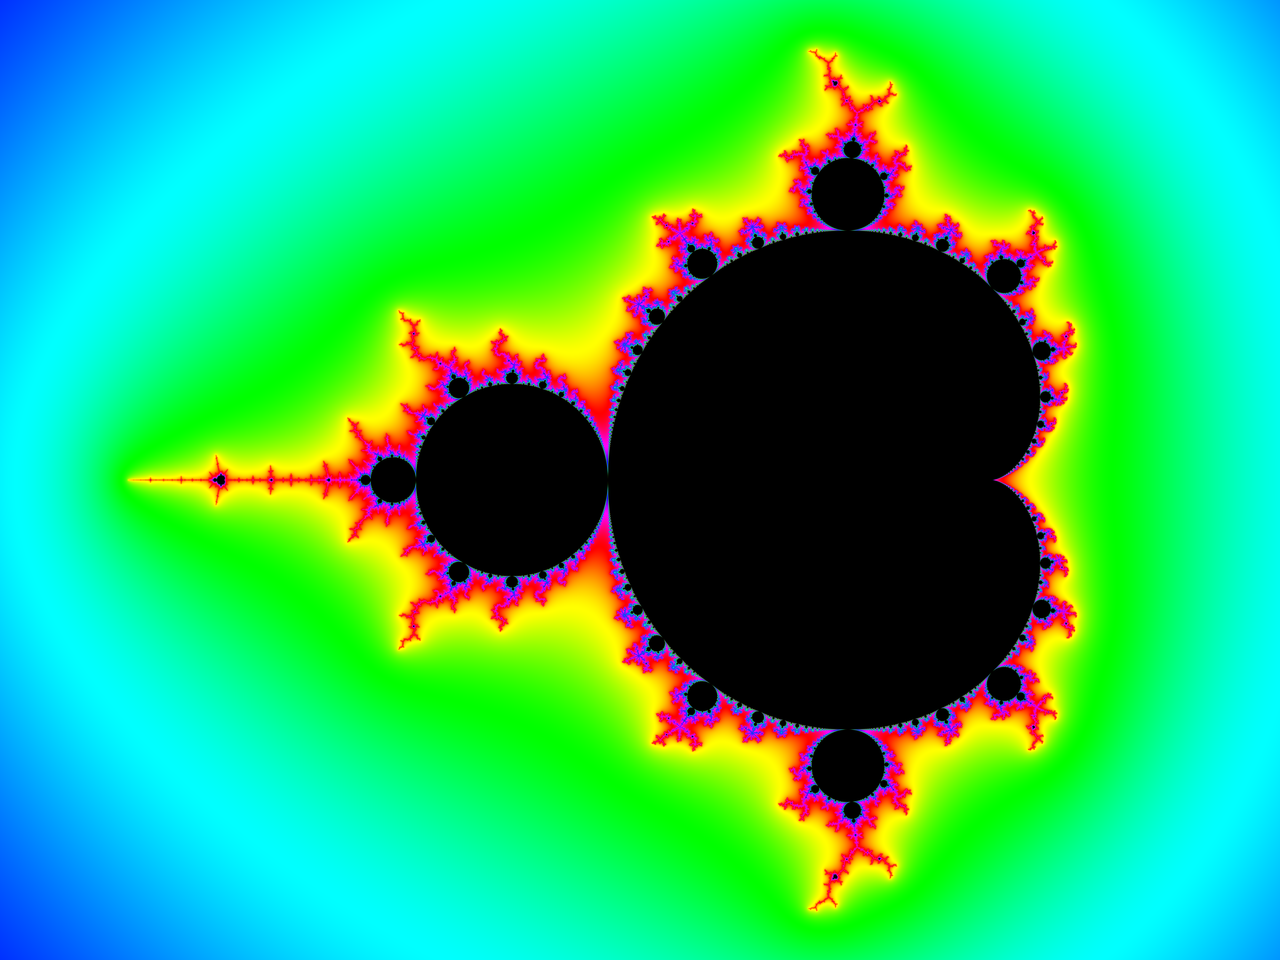
\includegraphics[width=.8\linewidth]{Bilder/mandelbrot}
	\bildquelle{Geek3, CC BY 3.0, \url{https://w.wiki/33UD}}
	\caption{Mandelbrot Rendering}
	\label{diesIstEinLabel} % Wichtig: Labels müssen immer UNTER dem Caption stehen!
\end{figure}

% Tipp für Wiki Quellen: https://meta.wikimedia.org/wiki/Special:UrlShortener


Mehrere Bilder in einer Abbildung sind auch möglich:

\begin{figure}[H]
	\centering
	\subfloat[Vogel\label{bild1}]{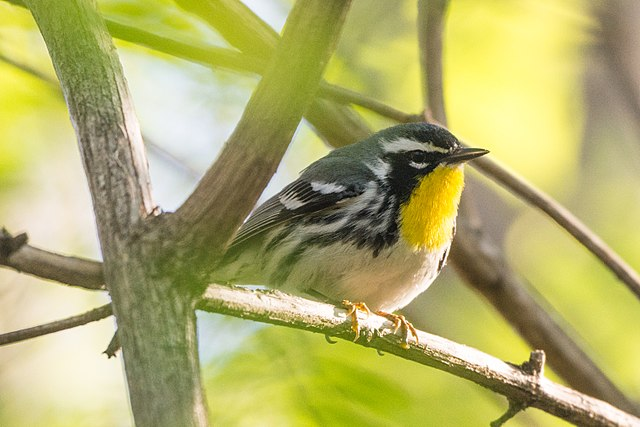
\includegraphics[width=0.45\linewidth]{Bilder/vogel}}%
	\qquad
	\subfloat[Kuh\label{bild2}]{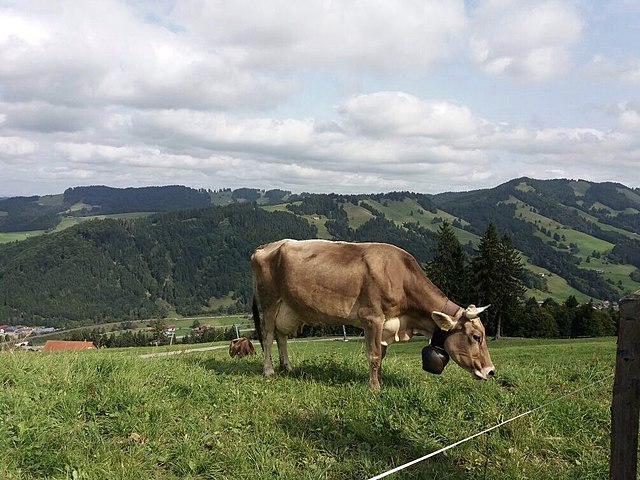
\includegraphics[width=0.45\linewidth]{Bilder/kuh
	}}%
	\bildquelle{\autoref{bild1}: Andrew C, CC BY 2.0, \url{https://w.wiki/33UJ}}
	\bildquelle{\autoref{bild2}: Killarnee, CC BY-SA 4.0, \url{https://w.wiki/33UK}}
	\caption{Verschiedene Bilder in einer Grafik}%
\end{figure}

Zum Zitieren wird der \lstinline|\cite{id}| Befehl verwendet. Dabei können auch Seitenzahlen angegeben werden, z.B. \cite{Haffner2018} oder \cite[S. 15]{Haffner2018}. Der Zitierstil ist in der \path{packages.tex} Datei definiert.

\section{Nützliche Tools}

\begin{itemize}
	\item Mathematische Symbole in Latex: \newline\url{https://detexify.kirelabs.org/classify.html}
	\item Bibliographieverwaltung: z.B. \url{https://www.jabref.org/}
	\item Tabellen: \url{https://www.latex-tables.com/}
\end{itemize}

Generell ist die Verwendung von GIT für die Arbeit zu empfehlen. Durch die Verwendung von Github / Bitbucket / Gitlab lassen sich automatisch Sicherungskopien erzeugen und Versionen verwalten.

%% Anhang
\appendix
\setcounter {chapter} {0}
\thumbchapter{Appendix}

\section{Anhang 1}

Dies ist er erste Anhang



% Literaturverzeichnis %%%%%%%%%%%%%%%%%%%%%%%%%%%%%%%%%%%%%%%%%%%%%%%%
\newpage

\bibliography{references}
\addcontentsline{toc}{chapter}{Literaturverzeichnis}
%% Anzeige der Quellen
\nocite{*} % Zeigt alle Quellen an, auch nicht zitierte. Falls nur zitierte Quellen angezeigt werden sollen, diesen Befehl entfernen
%%%%%%%%%%%%%%%%%%%%%%%%%%%%%%%%%%%%%%%%%%%%%%%%%%%%%%%%%%%
\end{document}

